\documentclass[]{article}
\usepackage{graphicx}
\usepackage{subfig}
\usepackage{amsmath}
\usepackage{amsfonts}
\newcommand{\pt}{\frac{\partial}{\partial \theta}}
\newcommand{\ptt}{\frac{\partial^2}{\partial \theta^2}}
\newcommand{\Ex}{\mathbb{E}}


\begin{document}
\title{CS689 Final Project:\\ Text Genre Classification in the $n <<p$ Regime}
\author{Sam Anzaroot and David Belanger}
\maketitle
\section{Introduction}

An overwhelming amount of text data becomes available every second. The text comes in chunks corresponding to articles, press releases, blog posts, tweets, etc. These can all be thought of in general terms as 'documents'. Suppose you are looking for particular information in a very large collection of documents. A common real world situation is that there are so many documents that the time cost of looking for the information in all of the documents is prohibitive. Many of these documents may be irrelevant, however. You aren't likely to find the latest information on the European economy by looking in the sports section of the Wall Street Journal, but looking in the main section would be fruitful. Here, there are underlying genres for documents given by the section of the newspaper that they appear in. In many settings, annotation of such underlying genres is not available explicitly, and we require automatic methods for discerning the genre of a do cument. 

Text genre classification can be accomplished by first mapping the document to a numerical feature representation and then using a general-purpose classification algorithm that was trained on labeled examples. Certain characteristics of text data make classification particularly challenging. These include:
\begin{enumerate}
\item Time has shown that the best way to embed documents in feature space is to map to a space where each dimension corresponds to a word in the vocabulary. The value in dimension $i$ for a document can be represented, for example, as the frequency of word $i$ appearing in the document [need a source for this]. Due to Zipf's law, the distribution of word usages in most text is extremely heavy-tailed [need a source for this]. Therefore, the dimensionality of the embeddings for documents in feature space can be quite high, in the tens of thousands. 
\item  In a given document, most words appear 0 times. Given that the feature embedding of documents has a dimension for each word, most dimensions are zero for a particular document. Therefore, features for text data are often extremely sparse. 
\item Data annotation can be expensive. Given the high dimensionality of feature embeddings for documents, we are often in the $n << p$ regime, where $n$ refers to the number of distinct training points and $p$ is the dimensionality of the feature space. 
\end{enumerate}
All three of these factors make classification difficult. Through experiments on the binary classification task of determining whether an article from Reuters is or isn't about corporate acquisitions, we help explain trends that occur when performing classification in this difficult regime. 
\section{Background}
\section{Experiments and Discussion}
Outline: 
I: c3.m plots (acc and time)
Observations: different algorithms have different behavior depending on size of training set. 
In figure ~\ref{fig:acc_vs_proj_dim} ...TODO. fix the figures too.


\begin{figure}[h!]
\centering
\subfloat[Naive Bayes]{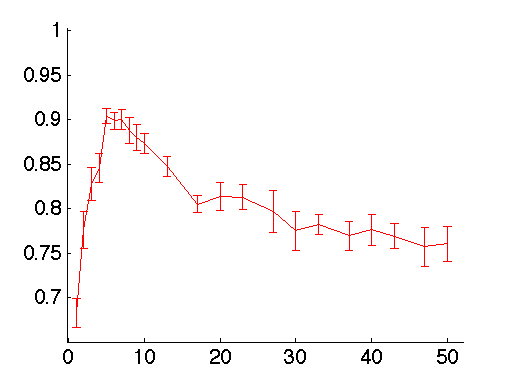
\includegraphics[width=.5\textwidth]{../images/nb_acc_vs_dim_pca_sr.png}}
\subfloat[SVM]{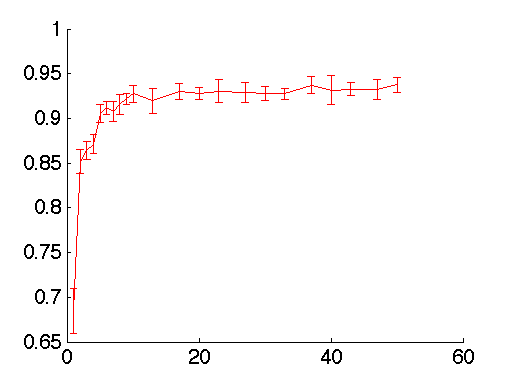
\includegraphics[width=.5\textwidth]{../images/svm_acc_vs_dim_pca_sr.png}}
\caption{Accuracy vs. dim. PCA Projection}
\label{fig:acc_vs_proj_dim}
\end{figure}

In analysis, here, mention something about how with svm model complexity scales with number of training examples, not dimensionality of feature space. Also, point out that it makes sense to use linear kernel, rather than rbf, because of COD. 

\begin{figure}[h!]
\centering
\subfloat[Reduced Data Sparsity]{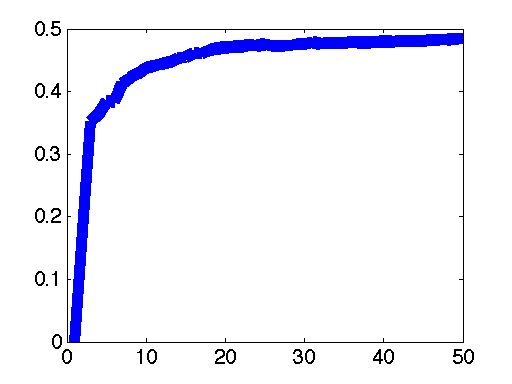
\includegraphics[width=.5\textwidth]{../images/PCAsparsityDensity.png}}
\subfloat[Cumulative Covariance]{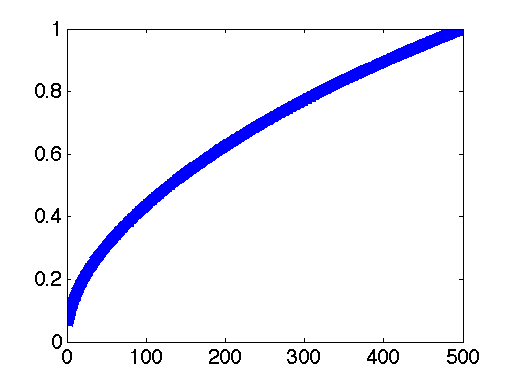
\includegraphics[width=.5\textwidth]{../images/pca_cumsum.png}}
\caption{Characteristics of PCA-reduced data}
\label{fig:PCA_RED}
\end{figure}

\begin{center}
\begin{figure}[h!]
\centering
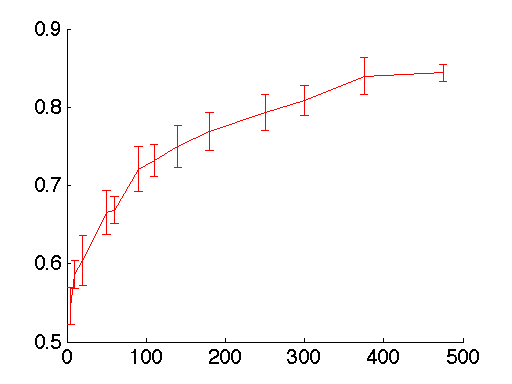
\includegraphics[width=.5\textwidth]{../images/accuracy_vs_dim_randproj.png}
\caption{Naive Bayes Acc. vs. num dim Rand. Projection}
\label{fig:myfig}
\end{figure}
\end{center}

%also include naive bayes small pca vs. naive bayes pca. If it was just an issue of underfit gaussians, nonsmall would do better for bigger training sets, but it doesn't. 

\begin{center}
\begin{figure}[h!]
\centering
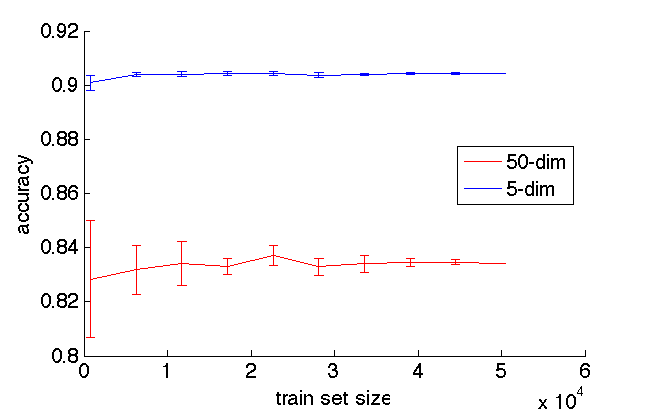
\includegraphics[width=.5\textwidth]{../images/nb_5_vs_50.png}
\caption{Naive Bayes Acc. vs. num dim Rand. Projection}
\label{fig:myfig}
\end{figure}
\end{center}


\begin{figure}[h!]
\centering
\subfloat[L1 regularization]{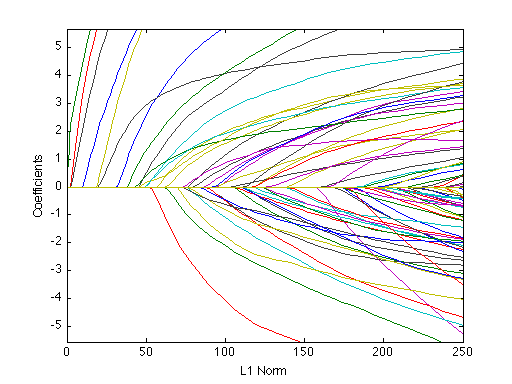
\includegraphics[width=.5\textwidth]{../images/lassoCoeffCurve.png}}
\subfloat[L2 regularization]{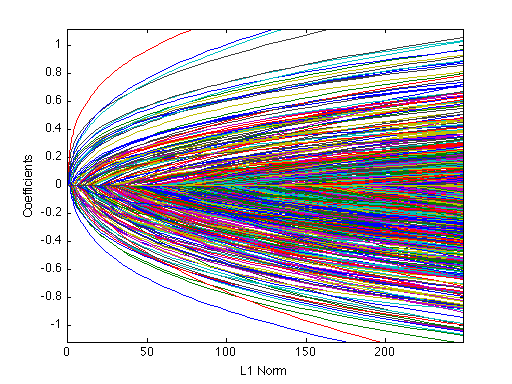
\includegraphics[width=.5\textwidth]{../images/ridgeCoeffCurve.png}}
\caption{Coefficient Paths for Regularized Logistic Regression}
\label{fig:PCA_RED}
\end{figure}


\end{document}

